\chapter{Graph}

\section{Basic}
\rih{Graph representation.} V for a vertex set with a map, mapping from vertex to its neighbors.
\begin{python}
V = defaultdict(list)
\end{python}

\section{BFS}
\subsection{BFS with Abstract Level}
Start bfs with a set of vertices in abstract level, not necessarily neighboring vertices.

Example:
$-1$ obstacles, $0$ targets, calculate all other vertices' Manhattan distance to its nearest target:
$$
\begin{bmatrix}
\infty & -1 & 0 & \infty \\
\infty & \infty & \infty & -1 \\
\infty & -1 & \infty & -1 \\
0 & -1 & \infty & \infty \\
\end{bmatrix} 
$$

is calculated as:
$$
\begin{bmatrix}
3 & -1 & 0 & 1 \\
2 & 2 & 1 & -1 \\
1 & -1 & 2 & -1 \\
0 & -1 & 3 & 4 \\
\end{bmatrix}
$$

\subsubsection*{Code}
\begin{python}
self.dirs = ((-1, 0), (1, 0), (0, -1), (0, 1))

def wallsAndGates(self, mat):
    q = [(i, j) for i, row in enumerate(mat) 
         for j, val in enumerate(row) if val == 0]
    for i, j in q:  # iterator
        for d in self.dirs:
            I, J = i+d[0], j+d[1]
            if (0 <= I < m and  0 <= J < n and 
                mat[I][J] > mat[i][j]+1):
                mat[I][J] = mat[i][j]+1
                q.append((I, J))
\end{python}



\section{Detect Acyclic}
\begin{enumerate}
\item \pythoninline{marked} is reset after a dfs. 
\item \pythoninline{visited} should be updated only in the end of the dfs. 
\item For directed graph:
\begin{enumerate}
\item Should dfs for all neighbors except for vertices in \pythoninline{visited}, to avoid revisiting. For example, avoid revisiting A, B when start from C in the graph $C \rightarrow A \rightarrow B$.
\item Excluding predecessor \pythoninline{pi} is erroneous in the case of $A \leftrightarrow B$ 
\end{enumerate}
\item For undirected graph:
\begin{enumerate}
\item Should dfs for all neighbors except for the predecessor \pythoninline{pi}. $A-B$.
\item Excluding neighbors in \pythoninline{visited} is redundant, due to \pyinline{pi}. 
\end{enumerate}
\end{enumerate}

\subsection{Directed Graph}

\begin{python}
def dfs(self, V, v, visited, pathset):
  if v in pathset:
    return False

  pathset.add(v)
  for nbr in V[v]:
    if nbr not in visited:
      if not self.dfs(V, nbr, visited, pathset):
        return False

  pathset.remove(v)
  visited.add(v)
  return True
\end{python}
\subsection{Undirected Graph}
\begin{python}
def dfs(self, V, v, pi, visited, pathset):
  if v in pathset:
    return False

  pathset.add(v)
  for nbr in V[v]:
    if nbr != pi:
      if not self.dfs(V, nbr, v, visited, pathset):
        return False

  pathset.remove(v)
  visited.add(v)
  return True
\end{python}

\section{Topological Sorting}
For a graph $G=\{V, E\}$, if $A \rightarrow B $, then $A$ is before $B$ in the ordered list. 
\subsection{Algorithm}
\rih{Core clues}:
\begin{enumerate}
\item \textbf{Dfs neighbors first}. If the neighbors of current node is  $\neg$visited, then dfs the neighbors
\item \textbf{Process current node}. After visiting all the neighbors, then visit the current node and push it to the result queue.

\end{enumerate}
Notice:
\begin{enumerate}
\item Need to check ascending order or descending order. 
\item Need to \textbf{detect cycle}; thus the dfs need to construct result queue and detect cycle simultaneously, by using two sets: $visited$ and $pathset$. 
\end{enumerate}
\begin{figure}[hbtp]
\centering
\subfloat{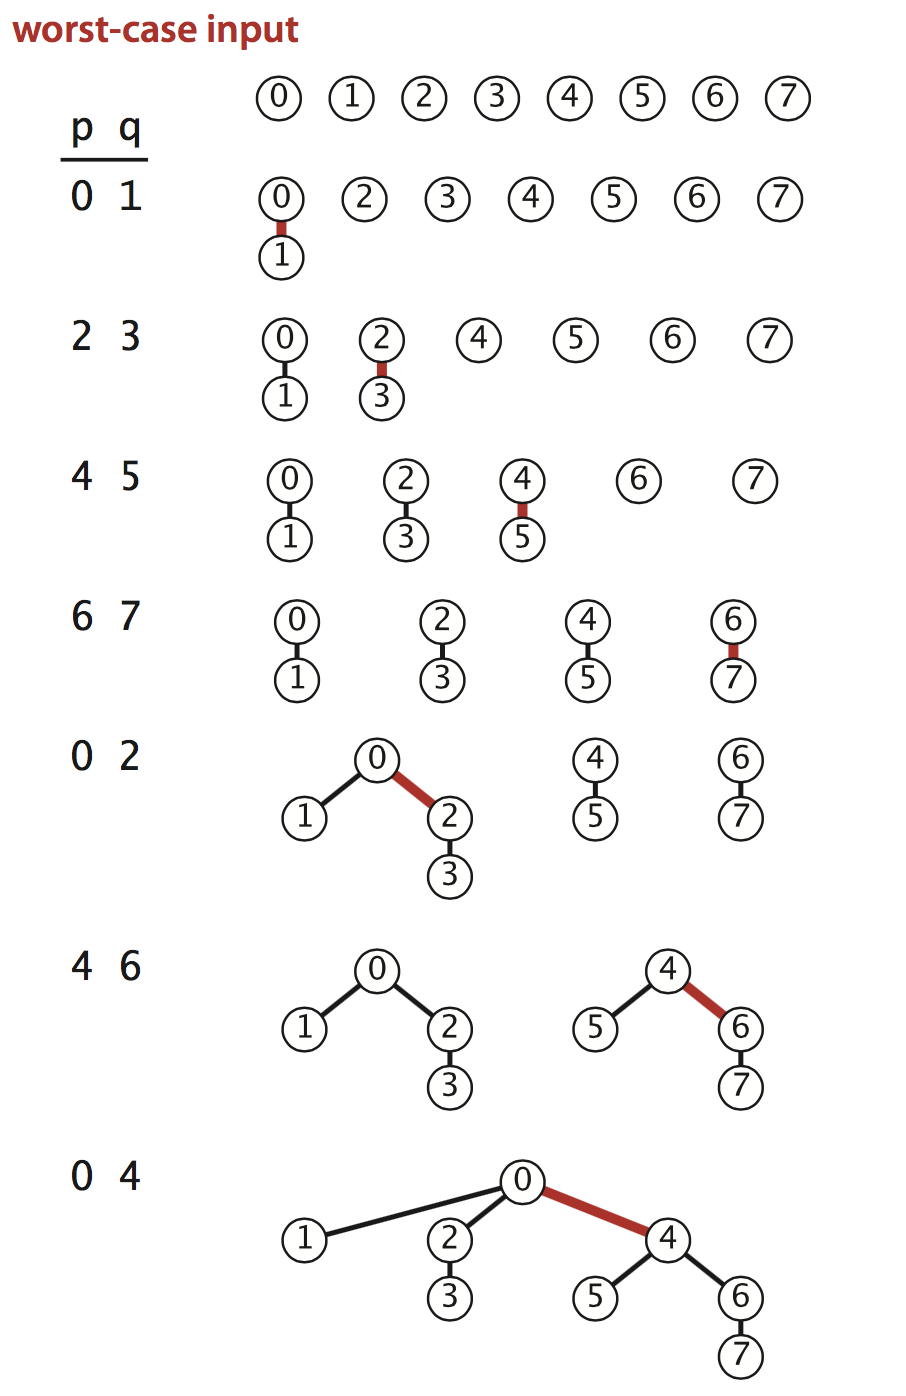
\includegraphics[scale=.70]{uf}}
\caption{Weighted quick-union traces}
\label{fig:union_find}
\end{figure}
\newpage
\begin{python}
from collections import deque

def topological_sort(self, V):
  visited = set()
  ret = deque()

  for v in V.keys():
    if v not in visited:
      if not self.dfs_topo(V, v, visited, set(), ret):
        return []  # contains cycle 

  return list(ret)

def dfs_topo(self, V, v, visited, pathset, ret):
  if v in pathset:
    return False

  pathset.add(v)
  for nbr in V[v]:
    if nbr not in visited:
      if not self.dfs_topo(V, nbr, visited, pathset, ret):
        return False

  pathset.remove(v)
  visited.add(v)
  ret.appendleft(v)
  return True

\end{python}

\subsection{Applications}
\begin{enumerate}
\item Course scheduling problem with pre-requisite. 
\end{enumerate}

\section{Union-Find}
Improvements:
\begin{enumerate}
\item Weighting: size-baladnced tree
\item Path Compression. 
\end{enumerate}}
\subsection{Algorithm}
Weighted union-find with path compression.\\
\rih{Core clues.} 
\begin{enumerate}
\item \textbf{$\pi$ array}:an array to store each item's predecessor pi. 
\item \textbf{Size-balanced}: merge the tree according to the size to maintain balance.
\item \textbf{Path compression}: Make the ptr in $\pi$ array to point to its root rather than its immediate parent. 
\end{enumerate}
\newpage
Code:
\begin{python}
class UnionFind(object):
    def __init__(self):
        self.pi = {}  # item -> pi
        self.sz = {}  # root -> size

    def __len__(self):
        """number of unions"""
        return len(self.sz)  # only root nodes have size

    def add(self, item):
        if item not in self.pi:
            self.pi[item] = item
            self.sz[item] = 1

    def root(self, item):
        pi = self.pi[item]
        if item != pi:
            self.pi[item] = self.root(pi)
            # path compression 
        return self.pi[item]

    def unionize(self, a, b):
        pi1 = self.root(a)
        pi2 = self.root(b)

        if pi1 != pi2:
            if self.sz[pi1] > self.sz[pi2]:
                pi1, pi2 = pi2, pi1
                # size balancing
            self.pi[pi1] = pi2
            self.sz[pi2] += self.sz[pi1]
            del self.sz[pi1]
        
    def is_union(self, a, b):
        if a not in self.pi or b not in self.pi:
          return False 
        return self.root(a) == self.root(b)
        
\end{python}

\subsection{Complexity}
$m$ union-find with $n$ objects: $O(n)+m O(\lg n)$

